%
%% Kapitel: Kapitel 4
%%======================================================================

\chapter{Auswahl der Simulationsumgebung}
\label{cha:Auswahl der Simulationsumgebung } \index{Einf{\"u}hrung in die Objekterkennung in Bildern}
%
%


Das Testen von Software f{\"u}r autonome Fahrzeuge in einer Simulationsumgebung (Software in the Loop) ist heute bereits zum Standard in der Automobilindustrie geworden.
Fahrsimulatoren stellen ein wichtiges Forschungs- und industrielles Entwicklungswerkzeug dar. Im Bereich der sicherheitsrelevanten Fahrerassistenzsysteme beginnt die Funktionsentwicklung verst{\"a}rkt mit Softwaremodellen. Software kann zu einem fr{\"u}hen Zeitpunkt in Fahrsimulatoren analysiert und Zusammenh{\"a}nge mit anderen Funktionen teilweise kosteng{\"u}nstiger als mit realen Prototypen untersucht werden. Die f{\"u}r einzelne Fragestellungen erforderlichen Fahrsituationen werden in einer Simulation gut kontrolliert und reproduzierbar dargestellt. Dabei besteht bei einer Simulation keine Gefahr f{\"u}r das reelle Fahrzeug. So lassen sich Pr{\"u}f- und Diagnose Software effizient auswerten. F{\"u}r das autonome Modellfahrzeug der Hochschule Karlsruhe soll deshalb eine geeignete Simulationsumgebung gefunden werden in der Bildverarbeitungs-Algorithmen und gesamte Softwarearchitekturen auf ihr Verhalten getestet werden k{\"o}nnen. Um die beste Wahl f{\"u}r das CaroloCup Team zu treffen wurde deshalb wieder eine Nutzwertanalyse der m{\"o}glichen Simulationsumgebungen erstellt. 
%[https://cuvillier.de/uploads/preview/public_file/2747/9783867277273.pdf]



\begin{figure}[H]
\begin{center}
  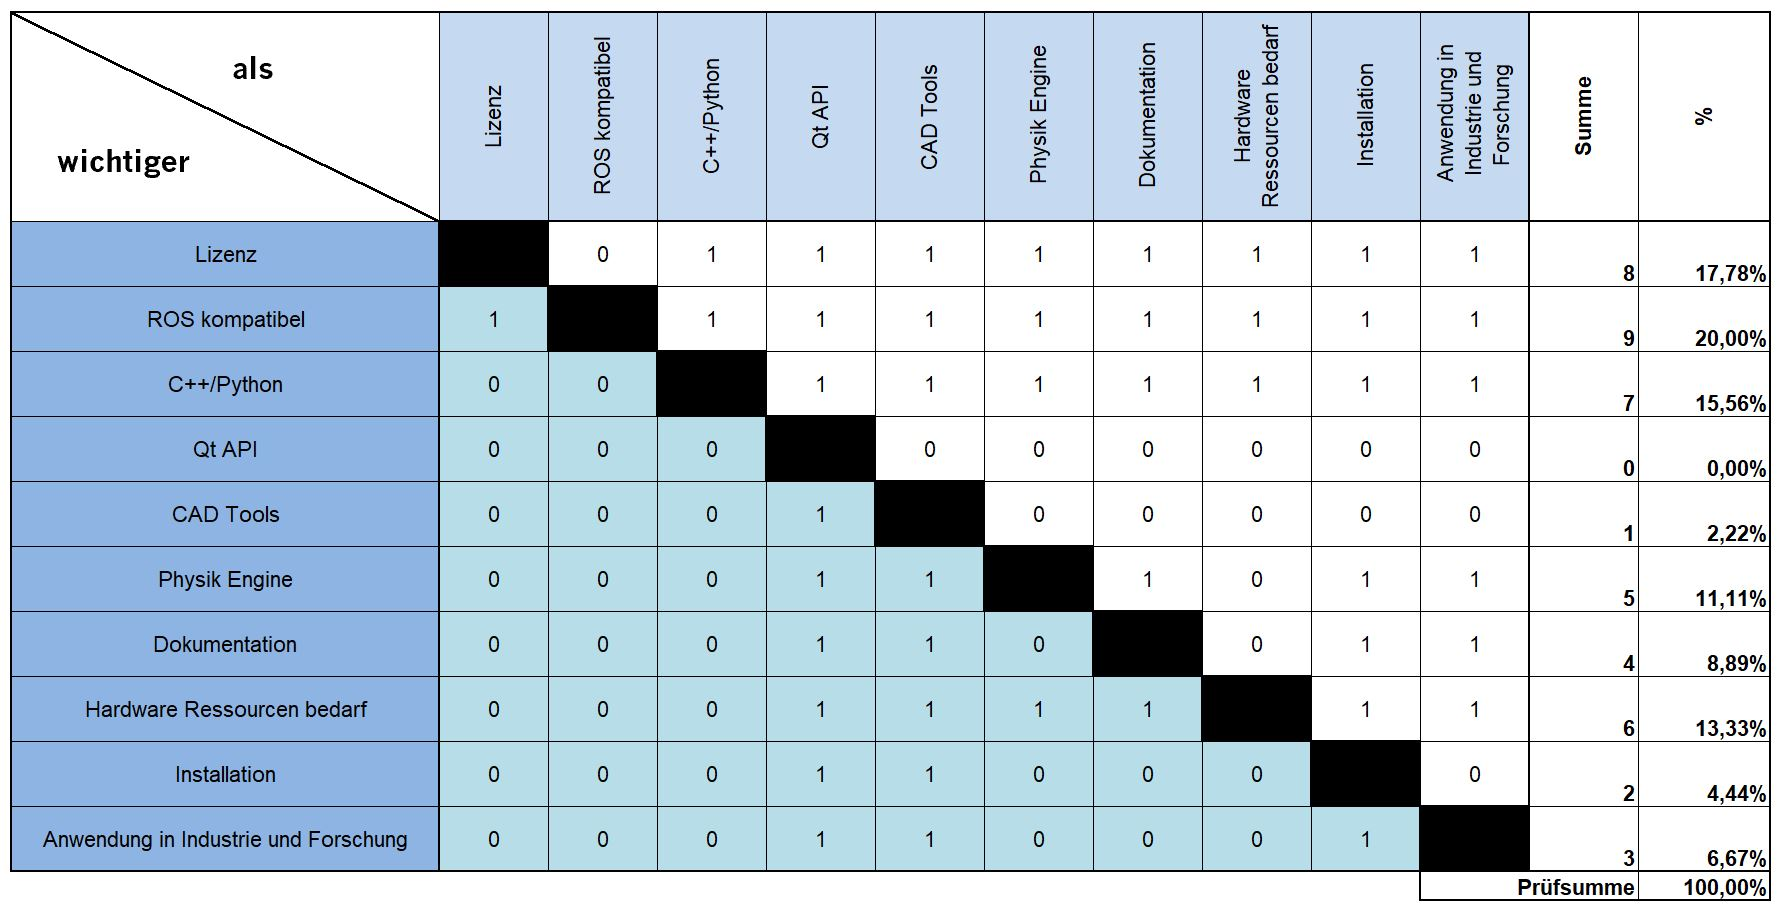
\includegraphics[width=1\textwidth]{/home/tb/Desktop/Master/BA_TB/02_Arbeit_Latex/005_Kapitel4/Bilder/paarweiser_vergleich_sim}% keine extention: w�hlt jpg f�r DVI
  \caption[Paarweiser Vergleich wichtiger Attribute einer Simulationsumgebung]%
           {\label{fig:PaarweiserVergleichSIM}%
           Paarweiser Vergleich wichtiger Attribute einer Simulationsumgebung.}
\end{center}
\end{figure}

Nach Auswertung des Paarweisen Vergleichs zeigt sich, dass vorallem die Kompatibilit{\"a}t zu ROS eine sehr wichtige Rolle bei der Auswahl der Simulaionsumgebung spielt.
Auch sollte die Simulationsumgebung keine kostenpflichtige Lizenz ben{\"o}tigen, da die Kosten nach CaroloCup-Regelwerk so niedrig wie m{\"o}glich gehalten werden sollen. Die Simulationsumgebung sollte auch eine C++- oder Python-API besitzen um das Fahrzeug mit der Bildverarbeitung zu koppeln.


\begin{figure}[H]
\begin{center}
  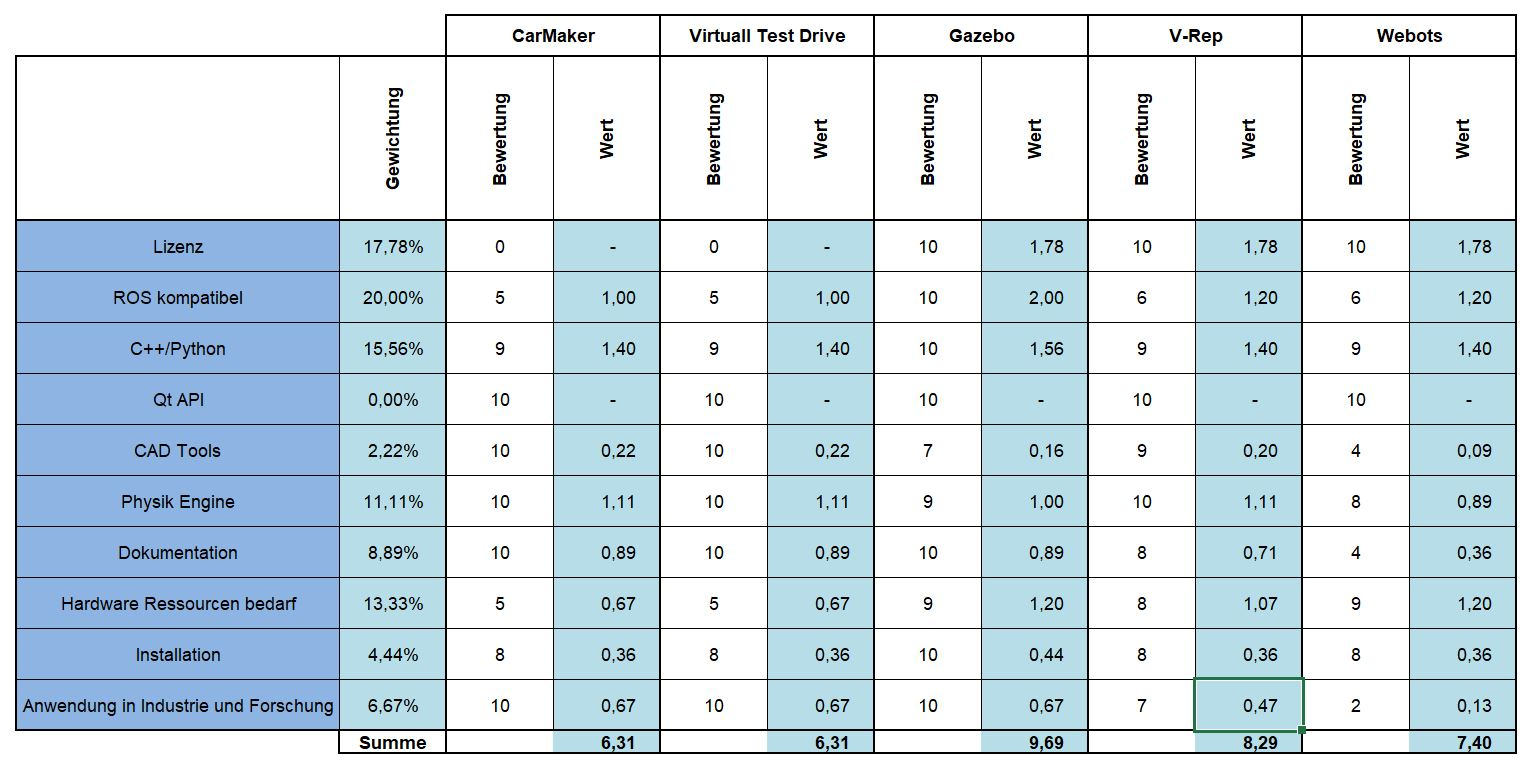
\includegraphics[width=1\textwidth]{/home/tb/Desktop/Master/BA_TB/02_Arbeit_Latex/005_Kapitel4/Bilder/nutzwertanalyse_sim}% keine extention: w�hlt jpg f�r DVI
  \caption[Auswertung der Nutzwertanalyse von verschiedenen Simulationsumgebungen]%
           {\label{fig:NutzwertAnalyseSIM}%
           Auswertung der Nutzwertanalyse von verschiedenen Simulationsumgebungen.}
\end{center}
\end{figure}

Die zwei Simulationsumgebungen mit der h{\"o}chsten Punktzahl (V-REP und Gazebo) sollen anschlie�end noch einmal n{\"a}her beschrieben werden.




\section{Die Virtual Robot Experimentation Platform Simulationsumgebung}
\label{sec:Die Virtual Robot Experimentation Platform Simulationsumgebung}
Die Virtual Robot Experimentation Platform (V-REP) ist eine dreidimensionale plattform{\"u}bergreifende Simulations-Engine von Coppelia Robotics. Sie unterst{\"u}tzt unter anderem C/C ++, Python, Lua, Octave und Matlab. Zur Simulation der Physik stehen verschiedene Engines zur Verf{\"u}gung, beispielsweise Newton, Bullet, Open Dynamics Engine oder Vortex.
Verf{\"u}gbar ist die Engine f{\"u}r MacOS, Linux und Windows.
V-REP bietet eine gro�e Auswahl an Robotern, einschlie�lich Bi-Pedal-, Hexapod-, Rad-, Flug- und schlangen{\"a}hnlichen Robotern. Zudem sind auch Aktoren und Sensoren, welche durch Plugins integriert werden k{\"o}nnen, verf{\"u}gbar.
Es gibt verschiedene Optionen f{\"u}r die Programmierung von Funktionen, wie etwa Skripte die Roboter ansteuern, Plugins und auch ROS-Knoten, die alle {\"u}ber die Remote-API eine Verbindung zu V-REP herstellen k{\"o}nnen
Vor allem bei der Konstruktion von neuen Robotern und Welten kann V-REP punkten.
Mit CAD designte Modelle k{\"o}nnen von Robotern in Echtzeit manipuliert werden.
Das Interagieren (z.B. verschieben oder hinzuf{\"u}gen) von Objekten wird erm{\"o}glicht. 
Es ist m{\"o}glich, Meshes zu vereinfachen, zu teilen und zu kombinieren. Meshes sind eine vereinfachte Oberfl{\"a}chenbeschreibungen aus dreidimensionalen Bilddateien. Dies erm{\"o}glicht es, die Dreieckszahl importierter Modelle zu optimieren und Meshes mit Roboteraktuatoren zu manipulieren \cite{simcomp}.


\section{Die Gazebo Simulationsumgebung}
\label{sec:Die Gazebo Simulationsumgebung}
Gazebo ist ein Open Source 3D-Simulator der f{\"u}r die Simulation von Robotern in verschiedenen, komplexen Szenarien erstellt wurde.
Begonnen hat die Entwicklung von Gazebo im Herbst 2002. Im Jahr 2009 wurde das Robot Operating System (ROS) in das Gazebo-Projekt integriert und ist seitdem eines der meistgenutzten Tools in der ROS Community. 2012 wurde die Verwaltung des Open-Source-Projekts Gazebo von der Open Source Robotics Foundation (OSRF) {\"u}bernommen und wird seitdem von OSRF und einer aktiven Community weiterentwickelt. 
Die Physik-Engines Open Dynamics Engine, Bullet, Simbody oder das Dynamic Animation and Robotics Toolkit k{\"o}nnen in Gazebo verwendet werden um die physikalischen Gegenbenheiten der Simulationsumgebung zu berechnen. Die Open Dynamics Engine ist in der Standardkonfiguration die aktive Physik-Engine.
Durch C++- oder Python-Plugins ist es auch m{\"o}glich Objekte oder die Physik zur Laufzeit der Simulation anzusteuern.
Verschiedene Sensor-Plugins sind in der Gazebo-ROS-API bereits integriert wie etwa Kamera-Sensoren oder eine Ackermann-Lenkung f{\"u}r Fahrzeuge.
Neben diesen Punkten bietet der Gazebo-Simulator viele Anwendungsbeispiele, von einfachen Einstiegsmodellen bis hin zu komplexen Modellen wie Roboterforschungsplattformen mit vielen verschiedenen Sensoren. Dies erm{\"o}glicht auch Entwicklern, die das Framework noch nicht kennen, einen schnellen Einstieg.
Gazebo nutzt unterschiedliche Software-Bibliotheken f{\"u}r die physikalische Simulation, das Rendering oder der Erzeugung von Sensordaten. Gazebo realisiert die Simulation {\"u}ber ein Client-Server Model.
Der gzserver ist f{\"u}r die Simulation der Physik das Rendering und dem Berechnen von Sensordaten zust{\"a}ndig. Der gzclient visualisiert die Simulation f{\"u}r den Benutzer. Durch diese Abstraktion ist es m{\"o}glich Gazebo headless (ohne grafische Ausgabe) laufen zu lassen. Dadurch wird die Simulation nicht visualisiert. Dies f{\"u}hrt zu einem niedrigeren Bedarf an Rechenressourcen.
Im Gegensatz zu V-REP bietet Gazebo weniger M{\"o}glichkeiten um Roboter in der Simulationsumgebung zu modellieren.
Die Modellierung in Gazebo kann {\"u}ber das SDF (Simulation Description Format), einem XML-Format zur Beschreibung
von Objekten und Umgebungen speziell f{\"u}r den Einsatz in der Robotersimulation bewerkstelligt werden. Dies ist f{\"u}r die Anforderungen des Wettbewerbsteams der Hochschule Karlsruhe vollkommen ausreichend.


%http://lenkaspace.net/tutorials/programming/robotSimulatorsComparison
%https://autonomesysteme.informatik.haw-hamburg.de/papers/2018Dannenberg.pdf


\section{Begr{\"u}ndung der Auswahl}
\label{sec:Begr{\"u}ndung der Auswahl}
Nach abwiegen aller Vor- und Nachteile der beiden Simulationumgebungen wurde sich f{\"u}r den Gazebo-Simulator entschieden. Die Hauptgr{\"u}nde daf{\"u}r waren, dass Gazebo schon bereits nativ mit ROS installiert wird. ROS-Gazebo-Plugins werden von den Entwicklern der Open Source Robotics Foundation betreut und sind daher wengier fehlerbehaftet. Gazebo stellt auch weniger Anforderungen an die Hardware Ressourcen im Gegensatz zu V-REP, dadurch k{\"o}nnte jedes neue Mitglied des Mechatronik Competition Teams Gazebo auf seinem eigenen Ger{\"a}t installieren. [Link hardware]
Die Kommunikation zwischen V-REP und ROS ist auch nicht von der selben Qualit{\"a}t wie der von ROS-Gazebo. Es ist nicht m{\"o}glich V-REP {\"u}ber Roslaunch-Dateien  aufzurufen. Zudem werden {\"u}ber die V-REP-ROS-API ROS-Nachrichten {\"u}ber ein LUA-Skript geparst was zu Performanznachteilen gegen{\"u}ber Gazebo f{\"u}hrt.



\section{Das SDF Format - System Description File}
\label{sec:Das SDF Format - System Description File}
SDF ist ein XML-Format, das Objekte und Umgebungen f�r Robotersimulatoren, Visualisierung und Steuerung beschreibt. Urspr{\"u}nglich als Teil des Gazebo-Robotersimulators entwickelt, wurde SDF unter Ber{\"u}cksichtigung wissenschaftlicher Roboteranwendungen entwickelt. Im Laufe der Jahre hat sich SDF zu einem stabilen, robusten und erweiterbaren Format entwickelt, das alle Aspekte von Robotern, statischen und dynamischen Objekten, Beleuchtung, Gel{\"a}nde und sogar Physik beschreiben kann.

\section{Das World File}
\label{sec:Das World File}
Das World File definiert durch SDF die zu simulierende Welt mit all ihren Komponenten. Es k{\"o}nnen Roboter oder Sensoren mit einer Welt verkn{\"u}pft, die Beleuchtung und Physikalischen Eigenschaft definiert, als auch statische Komponenten eingef{\"u}gt werden. Die World-Datei wird von dem gzserver eingelesen welcher nach den Definitionen die Welt generiert.



\section{Das Model File}
\label{sec:Das Model File}
Eine Modell-Datei beschreibt eine einzelne Einheit der Welt im SDF-Format. Dies k{\"o}nnte Beispielweise ein Fahrzeug f{\"u}r den CaroloCup sein. Einzelne Modell-Deteien k{\"o}nnen zusammen in ein World-File integriert werden.
Wie etwa verschiedene Fahrbahnsegmente.
Dies erm{\"o}glicht einen Modularen Aufbau und sorgt f{\"u}r bessere Lesbarkeit.
Die erste Hauptkomponente zum Beschreiben eines Modells ist der Link (<link>). Ein oder mehrere Links Formen ein Modell. Der Link kann viele verschiedene physikalische Attribute besitzen, wie die Masse (<mass>), das Tr{\"a}gheitsmoment(<inertial>) oder Reibwerte(<friction>). Des weiteren besitzt ein Link ein Kollisionsattribut (<collision>) wor{\"u}ber durch Angabe der geometrischen Gr{\"o}�e die Kollision mit anderen Komponenten der Welt errechnet wird. Eine weitere Komponente ist die visuelle Komponente(<visual>) sie kann optional die Geometrie des Links in der Simulation visualisieren. Auch Sensor-Komponenten(<sensor>) k{\"o}nnen in Links integriert werden, wie etwa ein Kamera-Sensor. Die zweite, optionale Hauptkomponente ist ein Gelenk (<joint>). Auch hiervon k{\"o}nnen mehrere in einem Modell existieren. Ein Gelenk verbindet zwei Links in einer Eltern-Kind-Beziehung miteinander. Verschiedene Gelenk-Typen k{\"o}nnen definiert werden wie etwa einem Drehgelenk(<jointtype=?revolute?>) f{\"u}r ein Rad oder ein Kugelgelenk (<jointtype=?ball?>) f{\"u}r eine Kamera. Durch Plugins(<plugin>) etwa geschrieben in C++ oder Python k{\"o}nnen zur Laufzeit verschiedene Funktionalit{\"a}ten f{\"u}r eine Simulation erg{\"a}nzt werden. Die R{\"a}der eines Fahrzeugs k{\"o}nnen dadurch angesteuert oder Kamera-Sensorwerte an eine ROS-Node {\"u}bermittelt werden \cite{gazebovrepeval}.



%https://autonomesysteme.informatik.haw-hamburg.de/papers/2018Dannenberg.pdf